\section{计算机基础知识}


开源排版系统\LaTeX{}与大家之前熟悉的软件有较多的不同,在使用过程中很可能遇到各种困难。没有任何编程基础的同学最好先阅读此部分。
\subsection{编译环境和代码编辑器}
常看到这样的提问“为什么我的\LaTeX{}界面和别人不一样?”,“非得安装TeXstudio吗?”,“安装完桌面为什么没有图标?”;学习LaTeX时也会碰到许多
相似的概念如\TeX{} Live,C\TeX{},xelatex,TeXworks等,使人感到迷惑。这些问题的根源在于,\LaTeX{}是一种计算机语言,与Word等软件并不一样,下面就来一一阐述。



\subsubsection{计算机语言}

人类社会有汉语,英语,法语等多种语言。然而,计算机并不能读懂人类的语言,要想指挥计算机完成各种任务,就要使用计算机语言。
计算机能直接识别运行的只有由0和1组成的二进制代码,称为\emph{机器语言},由于其可读性太差,科学家又创造了C,Java等采用
贴近人类语言的语法格式(主要是英语)描述程序的\emph{编程语言},并开发了对应的\emph{编译器},可以将编程语言翻译为计算机能识别的
二进制代码来运行,这个翻译的过程称作\emph{编译},在编译前的文件称为\emph{源代码}。

\LaTeX{}是一种宏语言,在排版时,通过各种各样的指令对文档的各种格式(比如字体,行距,居中,编号)进行控制,一份\LaTeX{}
源代码中既含有需要输出在文档中的具体内容,也含有控制指令。通过调用对应的\emph{编译器}进行\emph{编译},最后得到排版完成的PDF文档。
根据不同的需求,\LaTeX{}系统有不同的编译器,下面将其称为\emph{编译引擎}。主要有xelatex(主要处理中文文档),
pdflatex(主要处理英文文档),bibtex/biber(用于引入参考文献),lualatex等。我们说“采用xelatex方式编译文档”,指的就是
调用\emph{编译引擎}xelatex编译源代码文件。




\subsubsection{代码编辑器}


通过上面的介绍,你会发现,当你编写好代码后,要得到排版好的文件,起作用的其实是编译器,而采用什么样的代码编辑器
写源代码,其实是不重要的。实际上,如果你安装正确,你也可以使用记事本来编写代码,只要知道如何调用编译引擎。

那么代码编辑器有什么用呢?前面提到,代码需要通过编译才能得到我们要的PDF文档,但是,可能因为疏忽,编写某些指令有语法错误,
那么这个时候,编译就会报错,也就无法得到PDF文档(当然,有可能报错了,但是得到了正确排版的PDF文档)。此时就需要查找错误,
查找错误的过程被程序员称为\emph{Debug}。

如果使用记事本这种编辑器,你会发现查找错误非常痛苦,因为代码和你要排版的内容直接混在了一起,都是白纸黑字。许多代码编辑器
都含有\emph{语法高亮}的功能,会把不同的代码自动变成不同的颜色,这样,查找起来就比较方便了,语法高亮的效果如图(以VS Code为例)。
\begin{center}
  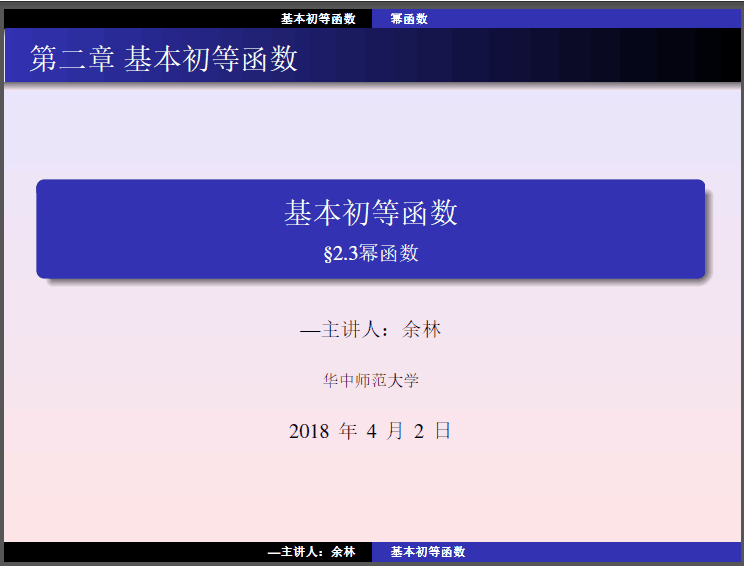
\includegraphics[scale=0.5]{1.png}
\end{center}

另一个重要的功能是\emph{语法补全},在输入各种指令时,非常容易打错,或者掉个把符号比如括号,许多代码编辑器在设定好你的编程语言后,
当你输入某些指令的前几个字符时,就会自动帮你联想可能的指令(很多时候就是你要的),这样就不容易打错,并且很多时候,插入"("等括号字符时,
会自动成对出现,避免漏掉。效果如图
\begin{center}
  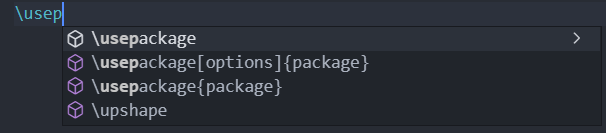
\includegraphics[scale=0.7]{2.png}
\end{center}

第三个方面是编译运行,\LaTeX{}有些代码编辑器如TeXstudio,不仅可以写代码,也提供了一键编译的按钮,如果你的编辑器没有编译的功能,就需要使用命令行编译(详见\ref{subsec:mlh}节),还有一些功能只能通过命令行使用。
这样对初学者来说上手起来就比较快。在安装\LaTeX{}时,一般会附带安装一个编辑器TeXworks,同样提供了高亮,补全,一键编译的效果,但整体比较简陋,没有
TeXstudio功能那么多,所以就会出现很多人推荐TeXstudio,导致很多人误解安装\LaTeX{}是安装TeXstudio。

个人比较喜欢的代码编辑器是VS Code,这是微软开发的开源编辑器,具有很强的自定义性,还有各种各样实用的插件,可根据自己的需求
配置各种指令和快捷键,不过编译环境需要自己配置,可以参考这个链接:\href{https://zhuanlan.zhihu.com/p/38178015?utm_source=qq&utm_medium=social&utm_oi=1122597840500740096}{使用VSCode编写LaTeX},
推荐对\LaTeX{}有一定了解后,再更换代码编辑器提高效率。



\subsubsection{发行版}


发行版指的是\LaTeX{}整个软件包的版本,\TeX{} Live,C\TeX{},MiK\TeX{}指的就是发行版,通常问安装哪个版本,指的是哪个发行版。有些模版和代码只能特定
的发行版下编译,比如本论文模版基于\TeX{} Live,邓老师的旧模板基于C\TeX{},不同的发行版通常不能兼容,因此
在一般情况下\emph{请勿安装超过一个发行版!}

一个发行版主要有三个部分:各种编译器,许许多多的宏包,宏包的说明文档。宏包可以理解为指令集,提供了更多的排版指令,当你需要对应指令时,只要加载对应
的宏包就可以调用许多方便的指令。

因此,你会发现其实安装\LaTeX{},是安装这一门语言的\emph{编译环境},使得你可以在自己的电脑上编译\LaTeX{}源文件。
前面说过,如果编辑器没有没有编译的功能,就需要使用命令行编译(详见\ref{subsec:mlh}节),本质是电脑运行程序的另一种方式。
因此,\emph{安装完成后,桌面没有图标!}需要自己尝试编译一个含中文的文件,如果编译成功,才能说明安装成功,或者依照手册《install-latex-guide-zh-cn》。




\subsection{命令行}\label{subsec:mlh}


\subsubsection{GUI与CLI}


我们现在的计算机操作用户界面采用图形方式显示,允许用户使用鼠标等输入设备操纵屏幕上的图标或菜单选项,这种界面称作\emph{图形用户界面(Graphical User Interface,简称GUI)}。
我们平常使用电脑主要都是在这样的界面进行的,通过鼠标打开文件,运行程序,非常方便。

\LaTeX{}是由美国计算机学家莱斯利·兰伯特(Leslie Lamport)在20世纪80年代初期开发的。在那个年代,图形界面的运用并不广泛,甚至鼠标也不普及,使用
最为广泛的用户界面是\emph{命令行界面(Command-line Interface,简称CLI)},这种界面通常不支持鼠标,用户通过键盘输入指令,计算机收到指令后,予以执行。

正是因为这样,\LaTeX{}是按照命令行界面的用户设计的,这就是为什么\emph{无论什么编译方式(包括Texstudio的一键编译),
其本质都是通过命令行运行指令调用相应的编译引擎},因此,我们需要学习一定的命令行知识。实际上,大部分的计算机语言都是类似这样,通过编译得到我们见到的软件。




\subsubsection{Windows 10系统下的命令行基本操作}\label{subsub:cz}


下面的操作均在Windows 10家庭版上完成,Mac和Linux上的操作类似。

在Windows中,命令行程序是“命令提示符”或“Windows Powershell”,可以利用菜单栏的搜索框(如图)查找。
\begin{center}
  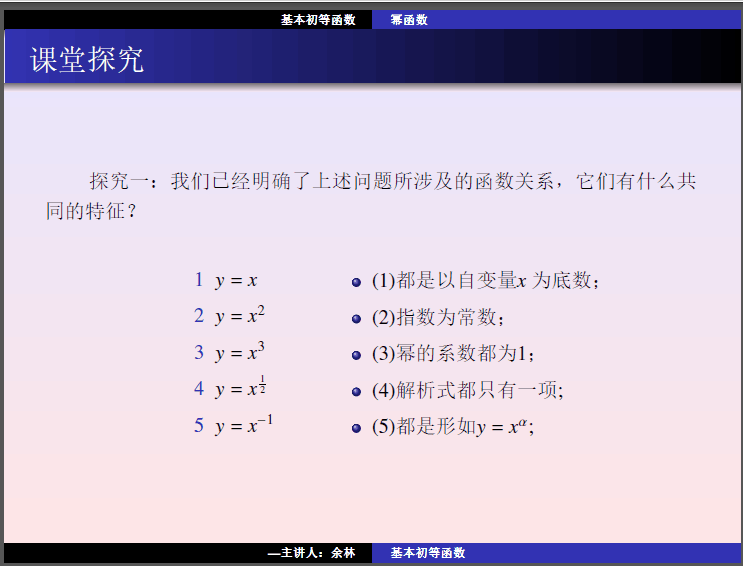
\includegraphics[scale=0.7]{3.png}
\end{center}运行时,建议右键选择“以管理员身份运行”,两个程序如图
\begin{center}
  
\includegraphics[scale=0.7]{4.png}
  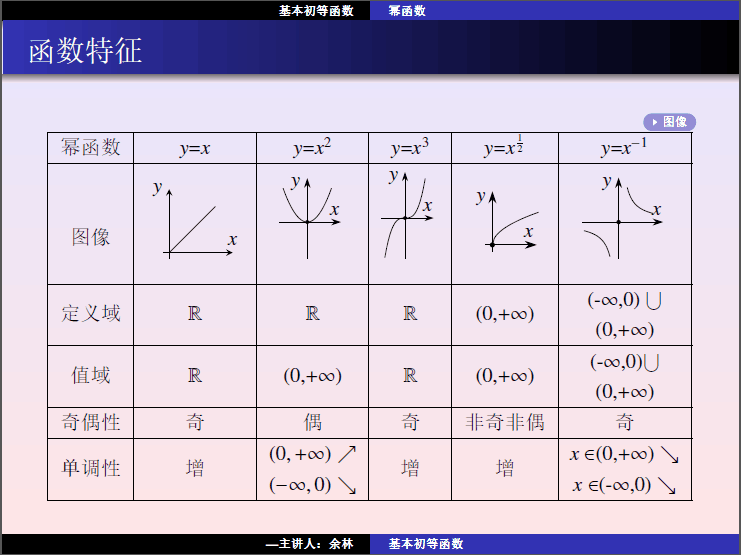
\includegraphics[scale=0.7]{5.png}
\end{center}

打开命令行窗口后(以“命令提示符为例”),会显示命令提示符(图中的红方框),由当前盘符、目录(即文件夹)和一个大于号>组成,
图中表示\emph{当前目录}为C盘WINDOWS文件夹下的system32文件夹。
\begin{center}
  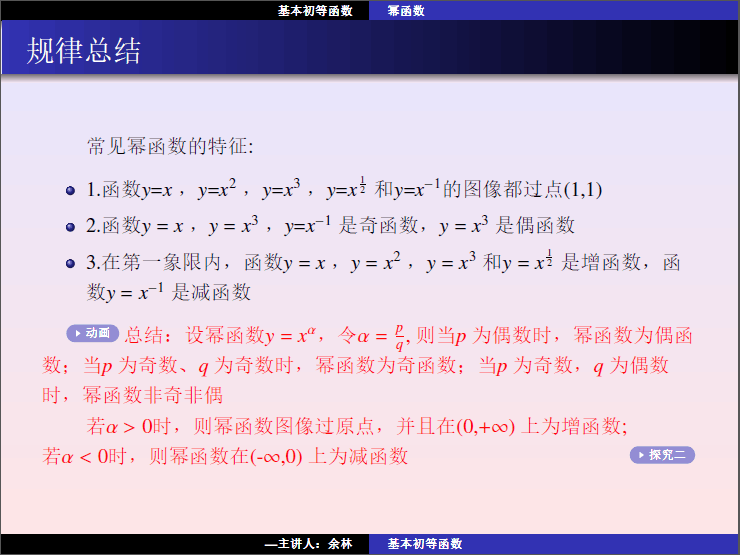
\includegraphics[scale=0.7]{6.png}
\end{center}
打开后在>的后面会有一个光标闪烁,等待输入命令,Windows命令行命令和文件名不区分大小写,输入一行
命令后按回车键执行,\emph{请注意把输入法调成英文半角,尤其是输入:和\texttt{\char92}的时候}。

下面以“用命令xelatex --shell-escape编译D盘下一个tex文件”为例进行演示

\emph{Step1:确定要编译的文件路径}

  首先找到你要编译的文件,在文件的目录的地址栏单击鼠标左键,被选中的部分就是这个文件的路径。
\begin{center}
  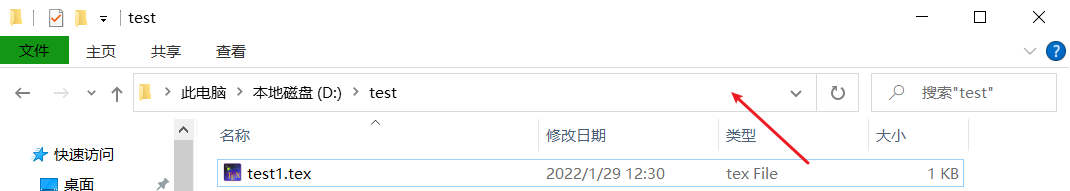
\includegraphics[scale=0.65]{7.png}
  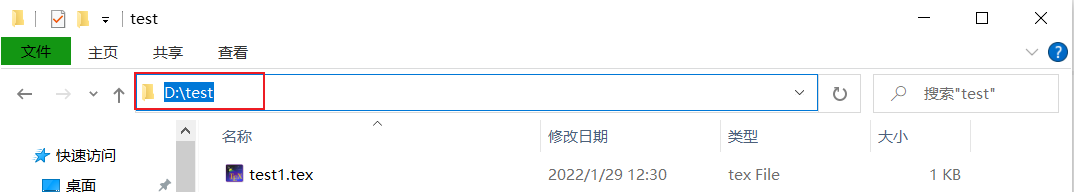
\includegraphics[scale=0.65]{8.png}
\end{center}
如图所示,源文件的存放路径是\verb"D:\test"

\emph{Step2:将命令行的当前目录切换为要编译的文件路径}

就像我们打开文件夹一样,\emph{只有命令行的当前目录为要编译的文件路径,才能进行编译},不然编译器根本找不到要编译的文件。

首先要从C盘更改为D盘,输入命令\verb"D:"后按回车键运行,会发现当前目录变成D盘。
然后输入命令\verb"cd \test"即可进入D盘下的test文件夹(目录)。
\begin{center}
  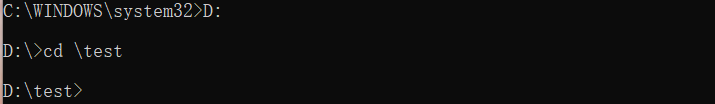
\includegraphics[scale=0.75]{9.png}
\end{center}

\emph{Step3:编译}

输入命令\verb"xelatex --shell-escape test1.tex"后按回车键开始编译,\verb"“test1.tex”"是要编译的文件的文件名。

\emph{等到再次出现命令提示符时}(如图所示),说明编译完成,此时可以回到原来的目录查看编译得到的PDF文件。
\begin{center}
  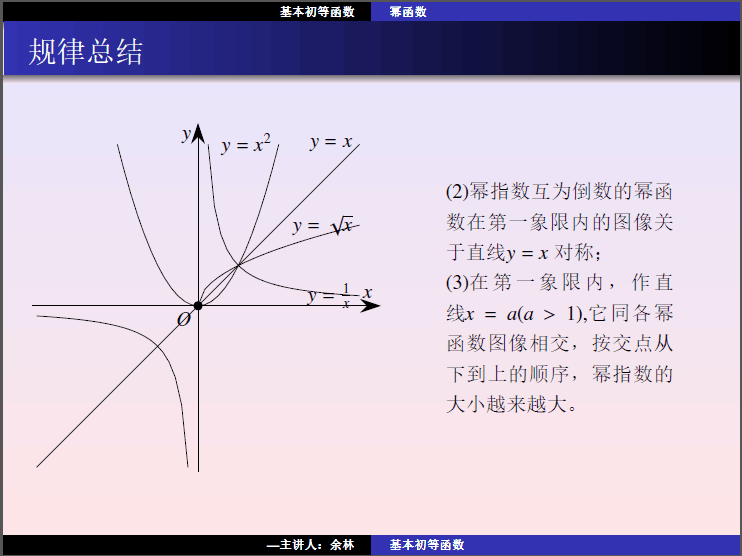
\includegraphics[scale=0.75]{10.png}
\end{center}

如果迟迟没有出现命令提示符,或者没有PDF文件,或者排版的效果非常奇怪,说明编写的代码有错误,需要进行排查。
可以阅读当前目录下生成的\verb"test1.log"日志文件,也可以直接阅读命令行窗口里的输出信息进行错误排查。由于报错
信息都是英语,需要随时准备使用翻译软件或者搜索引擎。

这个例子展示了命令行的基本用法,通过输入磁盘的字母和\verb"cd"指令进入需要运行命令的目录,再执行相应的命名,也有很多命令行
命令可以直接运行而不需要切换目录。希望大家看到“命令行下运行xx”这样的字眼时,能够不再害怕,而是上手操作。




\subsubsection{Windows Terminal}


使用命令行时每次都要手动切换目录未免让人感到厌烦,Windows 10 用户可以到微软商店(Microsoft Store)下载软件“Windows Terminal”。
安装完成后重新启动电脑,你会发现右键菜单增加了选项“Open in Windows Terminal”。

\begin{center}
  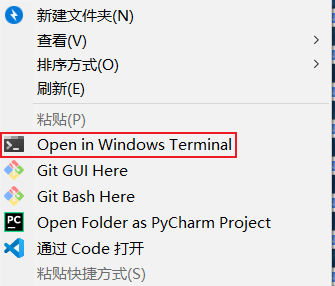
\includegraphics[scale=0.65]{11.png}
\end{center}
此时,只要在你需要进入的路径下按右键选择“Open in Windows Terminal”,弹出来的命令行窗口的当前目录就是你需要进入的路径!
但这种方式默认不是“以管理员身份运行”,因此,在一些情况下还是需要采用\ref{subsub:cz}节的方法。



\subsubsection{重要的环境变量Path}


你可能会想,能不能用命令行运行其他程序比如Word呢?然而,当你输入\verb"Word.exe"时,会得到如下的报错信息:\verb"'Word.exe'不是内部或外部命令,也不是可运行的程序或批处理文件。"

然而,你会发现,当你成功安装\LaTeX{}后,编译器的调用命令如\verb"xelatex,pdflatex"可以通过命令行在任意目录下使用;一些教程常常能看见这样的字眼“将xx添加到Path/环境变量”使人摸不着头脑,
其中的原因涉及到本节所讲的\emph{环境变量}。本节内容主要参考这个视频:\href{https://www.bilibili.com/video/BV1w741147G9?from=search&seid=9151606959931684460&spm_id_from=333.337.0.0}{『教程』什么是环境变量}。



\subsection{编码}


当你打开某些文件时,你可能发现眼前是完全无法阅读的一团乱码(比如用TeXstudio打开邓老师的旧模版),这里涉及到了编码的问题,
下面的介绍主要参考了这个视频:\href{https://www.bilibili.com/video/BV1ai4y1x7Uz?spm_id_from=333.999.0.0}{『教程』文字频频乱码 这背后是显卡的扭曲还是规则的沦丧?}

人类语言有各种各样文字,承载了大量的信息,那么如何在计算机中储存文字呢,由于计算机内部只有0和1,故问题转化为用数字表示文字,科学家通过建立数字和文字的一一映射,
比如英语是由26个字母组成的




\subsection{PDF阅读器}


PDF,全称为Portable Document Format,意为“可携带文档格式”,是由Adobe Systems用于与应用程序、操作系统、硬件无关的方式进行文件交换所发展出的文件格式。这种格式最大的优点在于,
不论在任何操作系统,手机还是电脑,最终的显示效果都是统一的,这就极大的方便了资料的传阅。\LaTeX{}代码在成功编译后,
得到的便是PDF文件,下面介绍几个PDF阅读器,用于满足两个需求,一是在写论文时随时编译查看效果,二是查看最终效果。



\subsubsection{Adobe Acrobat Reader}


Adobe Acrobat Reader是由PDF格式的设计公司Adobe推出的一款免费的PDF阅读器(请与收费的Pro版区分!)。这个阅读器的显示效果最好,且
支持PDF的所有功能(如JavaScript脚本、动画、3D对象等),\LaTeX{}的一些高级功能的效果只有使用这个阅读器才能完全显示。并且
可以查看PDF的许多属性比如使用的字体,在精细排版中会用到。

但有两个缺点,首先,安装时强制安在C盘,所以要记得腾空间。其次,\emph{Adobe Acrobat Reader会锁定PDF!在
Windows中重复编译时,要先关闭已经由Adobe Reader打开的PDF文档,否则PDF文件会被锁定而不能更新(同时会报错)},因此
一般在写论文途中采用其他的PDF阅读器。

下载地址:\url{https://www.adobe.com/cn/acrobat/pdf-reader.html}
\subsubsection{SumatraPDF}
SumatraPDF是一个很小的开源PDF阅读器,具有免安装版,可以放在U盘随身携带,并且打开速度非常快,适合在写作途中查看文档效果,
可以通过设置使得PDF可以反向搜索(定位到对应的代码)。当然,如果只是预览,Texwork编译后会自动弹出预览窗口。

下载地址:\url{https://www.sumatrapdfreader.org/download-free-pdf-viewer}\\或\url{https://sourceforge.net/projects/sumatrapdf-reader.mirror/}



\subsubsection{WPS}


WPS就不需要过多介绍了,与Office不同,它不强制安装在C盘。WPS包括了文字(Word),表格(Excel),演示(PPT)和PDF四个功能,安装好之后就可以直接阅读PDF文件。
顺带一提,WPS PDF可以给没有书签的PDF文档手动加书签(\emph{不需要会员!}),对于习惯使用电子书的同学会方便很多。

下载地址:\url{https://www.wps.cn/}